% !TEX root = ../thesis.tex
% !TEX spellcheck = en-US

\clearpage
\section{Experiments}

\subsection{TODO}

\begin{itemize}
  \item Comparison one-vs-rest and one-vs-one against linear machine
  \item Visualizations and embeddings of data in 2D (and decision boundaries?)
  \item show T-SNE embeddings of doc2vec vectors
\end{itemize}

\subsection{Effectiveness and Expressiveness of Statistical (Vector Space) Language Models}

\todo{say why using the sentence dataset here}
\todo{reference jupyter notebook here}
% http://localhost:8888/notebooks/thesis/experiments/vector-space-models/Vector%20Space%20Models.ipynb#Setup

As section \ref{sec:vector-space-models} explains, a popular way to approach text classification and other tasks in natural language processing is to build a language model by creating explicit representations of the objects or entities to be processed in a vector space. This way such vectors can be used as features and depending on the representation they can also encode notions of similarity of associativity between these objects.

In order to determine the most effective text representation, in a first set of experiments different approaches where studied and compared. Each method was studied with regards to the effect of its hyper-parameters on effectiveness when producing an input space to different classifiers, but also time and memory requirements at training and inference time are taken into account \todo{actually discuss time and memory requirements}.

\subsubsection{Baselines Classifiers: Uniform and Stratified Guessing}
\label{subs:baselines-classifiers}

As a baseline for comparing the performance of classification two different guessing strategies were used, namely uniform and stratified guessing. Uniform guessing refers to a predictor that samples from the given classes assuming a uniform distribution whereas stratified guessing takes the label distribution in the data as the underlying probability distribution and samples from it. Both, uniform and stratified guessing achieve a Matthews Correlation Coefficient score of around 0 (averaged over 1000 runs) as expected for such guessing strategies (see section~\ref{subs:informedness-markedness-mcc}). On the other hand the accuracy for uniform guessing is around 0.16 which corresponds to $1/\text{C}$ for the C classes and around 0.26 for stratified guessing which reflects the skew of the label distribution. Figure \ref{fig:exp-vector-space-conf-matrix-guessing} shows the confusion matrices for these baseline variants in absolute and normalized form which, clearly revealing the guessing strategies.

\begin{figure}[h]
 % From http://localhost:8888/notebooks/thesis/experiments/vector-space-models/Vector%20Space%20Models.ipynb#Baseline:-Guessing-Strategies
    \centering
    \begin{subfigure}[b]{0.47\textwidth}
        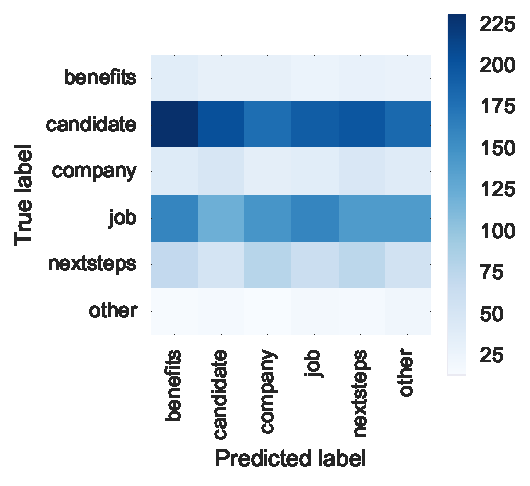
\includegraphics[width=\textwidth]{img/exp-vector-space-conf-matrix-guessing-uniform.pdf}
        \caption{Uniform}
      \label{fig:exp-vector-space-conf-matrix-guessing-uniform}
    \end{subfigure}
    ~
    %add desired spacing between images, e. g. ~, \quad, \qquad, \hfill etc.
    %(or a blank line to force the subfigure onto a new line)
    \begin{subfigure}[b]{0.48\textwidth}
        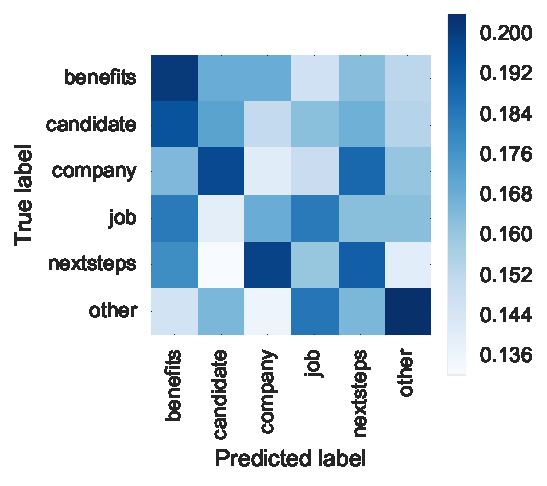
\includegraphics[width=\textwidth]{img/exp-vector-space-conf-matrix-guessing-uniform-normalized.pdf}
        \caption{Uniform (normalized)}
        \label{fig:exp-vector-space-conf-matrix-guessing-uniform-normalized}
    \end{subfigure}
    ~
    \begin{subfigure}[b]{0.47\textwidth}
        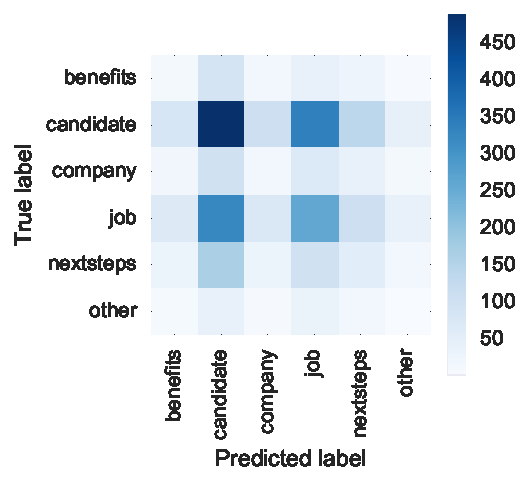
\includegraphics[width=\textwidth]{img/exp-vector-space-conf-matrix-guessing-stratified.pdf}
        \caption{Stratified}
        \label{fig:exp-vector-space-conf-matrix-guessing-stratified}
    \end{subfigure}
    ~
    %add desired spacing between images, e. g. ~, \quad, \qquad, \hfill etc.
    %(or a blank line to force the subfigure onto a new line)
    \begin{subfigure}[b]{0.48\textwidth}
        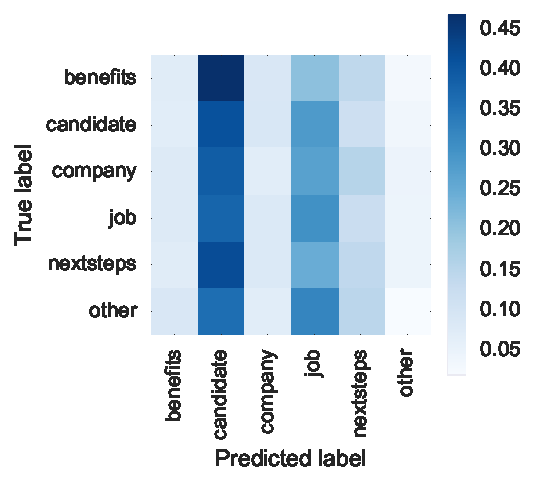
\includegraphics[width=\textwidth]{img/exp-vector-space-conf-matrix-guessing-stratified-normalized.pdf}
        \caption{Stratified (normalized)}
        \label{fig:exp-vector-space-conf-matrix-guessing-stratified-normalized}
    \end{subfigure}
    \caption{Confusion matrices of uniform and stratified guessing strategies. It  }
  \label{fig:exp-vector-space-conf-matrix-guessing}
\end{figure}

\subsubsection{N-gram Language Models}
\label{subs:n-gram-language-models}

The first class of language models that was investigated for the task of multi-class classification are N-gram models that were explained in section \ref{}



%
% \subsection{Classification of paragraph labels}
%
% \subsection{Unsupervised label detection}
%
%
%
% \subsection{Classification of sentence labels}
%
% \subsubsection{Experiment 1: Feature Extraction through Vector Space Models}
%
% \subsubsection{N-gram models}
% \label{ngram-models}
%
%
%
% \subsubsection{Distributed Representations language models}
% \label{doc2vec}
%
% Following an approach proposed by \cite{Le:2014aa}, the rationale of this experiment was to find out it was possible to obtain a more expressive language model than the N-gram based methods described in \ref{ngram-models}.
%
% The idea is based
%
% \subsection{Neural Networks}
